% !TEX encoding = UTF-8
% !TEX TS-program = pdflatex
% !TEX root = computabilità e algoritmi.tex
% !TEX spellcheck = it-IT
\chapter{Algoritmi multithread}\label{algoritmi-multithread}

Finora abbiamo visto solamente algoritmi sequenziali, ma il progresso ha fornito la possibilità di eseguire algoritmi paralleli.

Il problema è che non c'è un modello di calcolo preciso. 
Tipicamente ci sono più processori con della memoria condivisa, oppure ci sono dei cluster composti da processori, ognuno con la propria memoria che comunica con altri cluster per condividere i dati.

Noi ci limiteremo al caso con più processori con memoria condivisa.

In questo caso il lavoro deve essere distribuito tra i vari processori, utilizzando dei \textbf{thread}, dei processi logici che vengono assegnati ai vari processori.

Tipicamente una volta che il thread è stato avviato, questo non viene fermato e rimane in esecuzione su quel processore fino alla fine (\textbf{thread statico}).

La gestione dei thread viene effettuata in modo automatico (\textbf{threading dinamico}) perché lasciarla allo sviluppatore è troppo pericoloso. 
Con questa modalità, il programmatore può specificare quali parti del programma possono essere eseguite in parallelo, la suddivisione del programma in thread viene lasciata alla \textbf{piattaforma parallela} i quali vengono poi assegnati ai vari processori.

L'assegnazione viene effettuata con uno scheduler che cerca di bilanciare il lavoro svolto dai vari processori.

\section{Il primo algoritmo parallelo}\label{il-primo-algoritmo-parallelo}

Come notazione per lo pseudo codice utilizzeremo:

\begin{itemize}
\item
  \textbf{spawn}: posta davanti ad un istruzione indica che questa può essere eseguita in parallelo rispetto al resto del programma. In altre parole segnala che l'istruzione può essere eseguita su un altro thread.
\item
  \textbf{sync}: segnala che è necessario aspettare la terminazione di tutti i thread attivati con spawn.
\item
  \textbf{parallel}: specifica che il corpo di un ciclo \texttt{for} può essere eseguito in modo parallelo.
\end{itemize}

L'istruzione \textbf{spawn} non obbliga il sistema ad eseguire il codice in parallelo, è il sistema che sceglie se conviene o meno.

Se da un programma parallelo togliamo tutte queste istruzioni, otteniamo un classico programma sequenziale.

\subsection{Fibonacci ricorsivo}\label{fibonacci-ricorsivo}

\begin{breakablealgorithm}
\caption{P-Fib: fibonacci in versione parallela}
\begin{algorithmic}[1]
\Function{P-Fib}{n}
\If{$n \leq 1$}
    \State \Return $n$
\EndIf
\State $x \gets \textbf{ spawn } \textsc{P-Fib}(n-1)$ 
\State $y \gets \textsc{P-Fib}(n-2)$
\State $\textbf{sync}$
\State \Return $ x + y$
\EndFunction
\end{algorithmic}
\end{breakablealgorithm}

La complessità per la \textbf{versione sequenziale} di questo codice è proporzionale al numero ritornato dalla funzione, il quale cresce esponenzialmente.

\subsection{Grafo di computazione}\label{grafo-di-computazione}

L'esecuzione di un algoritmo multithread può essere rappresentata con un DAG.

Come prima cosa è necessario individuare gli \textbf{strand} ovvero le porzioni di codice che vengono eseguite in modo sequenziale.

Come notazione per il grafo viene utilizzato:

\begin{itemize}
\item
  \textbf{nero} o un pallino pieno per indicare uno strand.
\item
  \textbf{grigio} o un pallino con una crocetta per indicare la porzione di codice che c'è tra una \textbf{spawn} e una \textbf{sync}.
\item
  \textbf{bianco} o un pallino vuoto per indicare l'istruzione di
  ritorno per un thread (o funzione).
\end{itemize}

\begin{figure}[htbp]
\centering
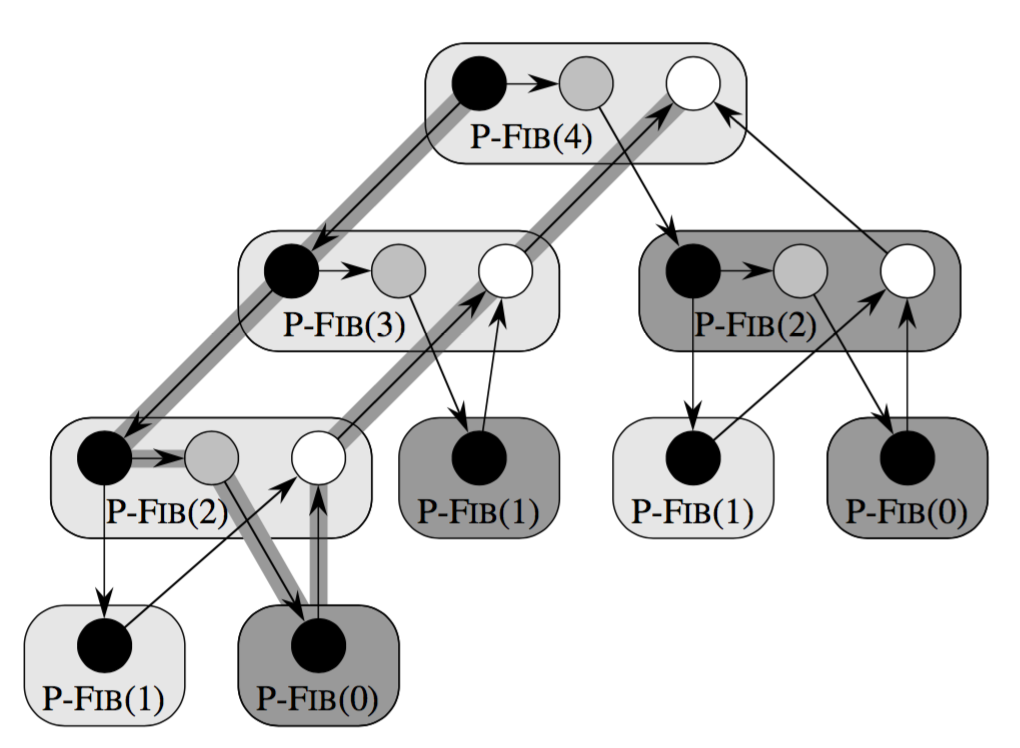
\includegraphics[width=.6\textwidth]{./notes/immagini/l24-fig1.png}
\caption{DAG per \textsc{P-Fib}(4)}
\end{figure}

Nel DAG sopra riportato gli archi hanno vari significati:

\begin{itemize}
	\item \textbf{archi di continuazione}: sono quelli orizzontali che connettono uno strand a quello successivo all'interno della stessa procedura.
	\item \textbf{archi di spawn}: sono quelli che vanno verso il basso e rappresentano il fatto che uno strand ha richiesto lo spawn di un altro strand.
	\item \textbf{archi di chiamata}: anche questi vanno verso il basso e rappresentano l'invocazione di un'altra funzione. Nel grafico fatto dal professore rimangono interni allo stesso blocco.
	\item \textbf{archi di ritorno}: sono quelli che vanno verso l'alto e rappresentano la terminazione di una funzione.
\end{itemize}

\begin{figure}[htbp]
	\centering
	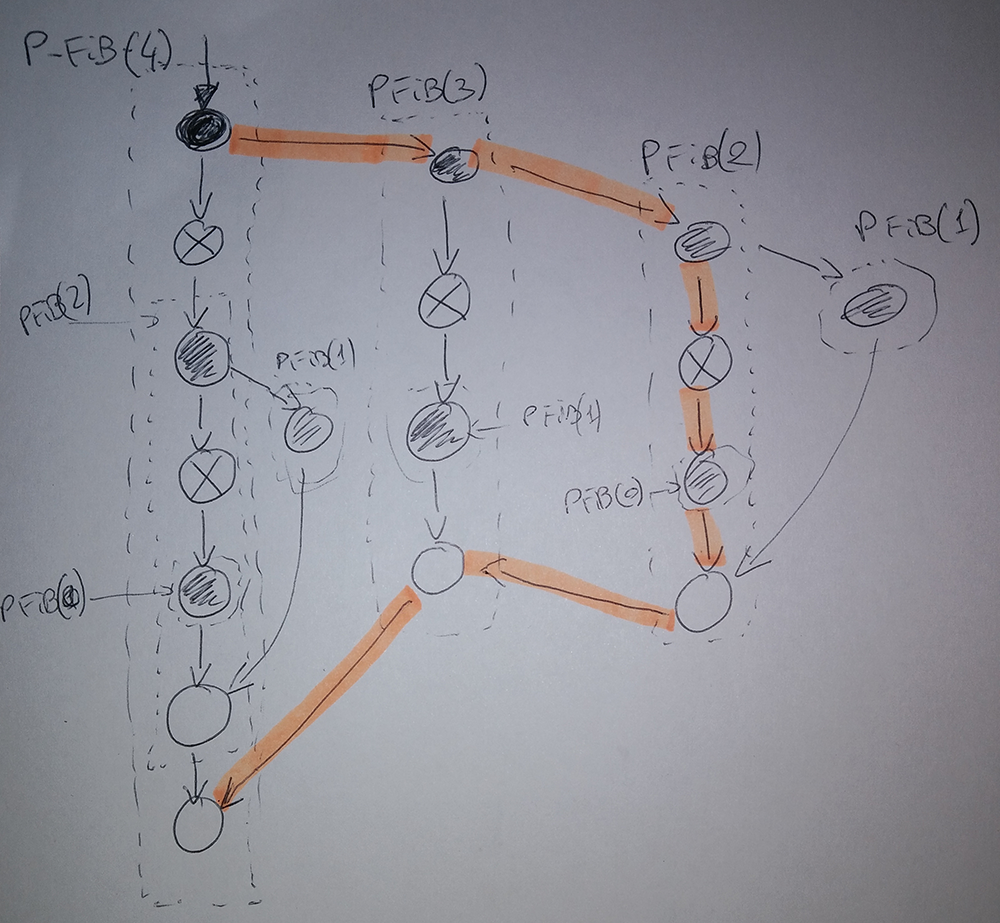
\includegraphics[width=.6\textwidth]{./notes/immagini/l24-alt.png}
	\caption{DAG per \textsc{P-Fib}(4) rappresentato come ha fatto il prof. Anziché evidenziare le chiamate delle funzioni, vengono evidenziati i possibili thread.}
\end{figure}

\subsection{Metriche per la complessità}\label{metriche-per-la-complessituxe0}

Per quanto riguarda la complessità asintotica possiamo considerare che l'esecuzione di uno strand avvenga in tempo costante.

Vengono poi distinte due misure: il \textbf{lavoro} ovvero il numero di strand e la \textbf{durata} (span) che è la lunghezza del cammino massimo (critico) del DAG, ovvero il numero di strand che devono per forza essere eseguiti in sequenza.

Nell'esempio di Fibonacci, il lavoro è 17 e la durata è 8 unità di tempo.

Ovviamente se l'algoritmo viene eseguito in modo sequenziale, il lavoro coincide con la durata ($T_1$). 
Se invece si hanno a disposizione infiniti processori, la durata è il tempo minimo richiesto ($T_\infty$). 

Infine, se si hanno a disposizione \emph{P} processori, valgono:

\begin{itemize}
	\item \textbf{legge del lavoro}: $T_P \geq \frac{T_1}{P}$ che deriva dal fatto che idealmente un computer con \textit{P} processori in $T_P$ riesce a produrre un lavoro pari a $P T_P$
	\item \textbf{legge della durata}: $T_P \geq T_\infty $ che deriva dal fatto che un computer con $P$ processori non può andare più veloce di un computer con processori illimitati.
\end{itemize}

Lo \textbf{speedup} di un algoritmo misura quanto viene velocizzato l'algoritmo utilizzando \emph{P} processori al posto di uno solo: 

$$\textbf{speedup} = \frac{T_1}{T_P} \leq P$$

Se lo speedup è molto più piccolo di \emph{P} non è conveniente aumentare il numero di processori.

Lo speedup viene detto \textbf{lineare} se

$$\frac{T_1}{T_P} = O(P)$$

e \textbf{perfetto} se

$$\frac{T_1}{T_P}  = P$$

Un'altra misura è data dal \textbf{parallelismo} che è il rapporto tra $T_1$ e $T_\infty$ e misura il lavoro medio che può essere eseguito in parallelo, fornendo un limite superiore per lo speedup.

Il parallelismo fornisce anche un limite allo speedup perfetto, ovvero supponendo di avere un numero di processori molto più grande del parallelismo ($P > T_1 / T_\infty$):

$$
T_1/T_P \leq T_1/T_\infty < P
$$

e quindi se 

$$P \gg \frac{T_1}{T_\infty} \quad \text{ allora } \quad \frac{T_1}{T_P} \ll P$$

più processori si hanno rispetto il parallelismo, peggiore è lo speedup. Questo perché avere un numero di processori maggiori rispetto al parallelismo implica che alcuni di questi rimarranno inattivi, ovvero non contribuiscono ad abbassare $T_P$.

Il \textbf{lasco} del parallelismo viene definito come

$$\frac{T_1/T_\infty}{P}$$

ovvero di quanto il parallelismo è maggiore del numero di processori.

Se il lasco è minore di 1, si ha che 

$$\frac{T_1}{T_P} \leq \frac{T_1}{T_\infty} < P$$

e quindi lo speedup non potrà mai essere perfetto. 

Se invece il lasco è maggiore di 1, ci si può avvicinare allo speedup perfetto.

\subsection{Lo scheduling dei thread}\label{lo-scheduling-dei-thread}

L'ordine ottimo che minimizza la durata dell'algoritmo è dato dall'ordinamento topologico del DAG, ma dal momento che il DAG non è noto a priori, non è possibile calcolarlo.

Lo scheduler più semplice è quello \textbf{goloso}, il quale assegna il maggior numero possibile di strand ai processori che ha a disposizione. Se ci sono più strand che thread, la scelta degli strand da assegnare viene fatta casualmente.

Se tutti i thread sono in esecuzione si verifica un passo \textbf{completo} ovvero tutti i processori stanno lavorando. 
Se non ci sono strand a sufficienza per tenere impegnati tutti i processori si ha un passo \textbf{incompleto}. 
Si ottiene così una durata che è pari alla somma dei passi completi e di quelli incompleti.

\subsubsection{Durata di un algoritmo con lo scheduler goloso}

Usando lo scheduler goloso è sempre vero che:

$$T_P \leq \frac{T_1}{P} + T_\infty$$

Il numero di passi completi è $\leq \frac{T_1}{P}$, perché se per assurdo non lo fosse, verrebbe eseguito più lavoro di quanto necessario:

\begin{align*}
\underbrace{P \cdot \bigg(\bigg\lfloor \frac{T_1}{P}\bigg\rfloor +1 \bigg)}_{\text{lavoro svolto dai passi completi assumendo di farne più del necessario}} &= P \bigg( \frac{T_1}{P} - (T_1 \mod P) +1 \bigg) \\
&= T_1 - (T_1 \mod P) + P \\
&> T_1
\end{align*}

 il che è assurdo, perché verrebbe svolto più lavoro del necessario.

Dopo aver eseguito un certo numero di passi completi, verrà eseguito un passo incompleto, quando questo succederà il DAG della computazione sarà un grafo $G'$ che avrà un numero di nodi iniziali (senza dipendenze) minore di \emph{P}, perché il passo è incompleto. 
Per forza di cose, uno di questi nodi appartiene al cammino critico e verrà eseguito, diminuendo di 1 la lunghezza di tale cammino. 
Dal momento che all'inizio la lunghezza del cammino è $T_\infty$, possono esserci al massimo
$T_\infty$ passi incompleti.

Quindi, dato che un passo può essere o completo o incompleto, la durata dell'algoritmo con $ P $ processori è limitata dal numero di passi, ovvero:

$$
T_P \leq \underbrace{\bigg\lfloor \frac{T_1}{P}\bigg\rfloor}_{\text{massimo numero di passi completi}} + \underbrace{T_\infty}_{\text{massimo numero di passi incompleti}}
$$

Questo tipo di scheduler funziona sufficientemente bene dal momento che nel caso peggiore richiede il doppio del tempo rispetto alla schedulazione ottima effettuata conoscendo a priori il DAG, ovvero lo scheduler goloso è \textbf{2-competitivo}.

Sia $T_{P}^*$ il tempo richiesto dallo scheduler ottimo, si ha che per le leggi della durata e del lavoro:

$$T_{P}^* \geq \max \bigg( \frac{T_1}{P} \: , \: T_\infty \bigg)$$

Si ha quindi 

\begin{align*}
T_{P} &\leq T_1/P + T_\infty \\
		 &\leq 2 \cdot \max \bigg( \frac{T_1}{P} \: , \: T_\infty \bigg) \\
		 &\leq 2T_{P}^*
\end{align*}

Inoltre, se $ P \ll T_1 / T_\infty $ si ha che $ T_P \approx T_1/P$, ovvero lo scheduler goloso riesce ad approssimare il parallelismo perfetto al crescere del lasco.

Questo perché se $ P \ll T_1 / T_\infty $ si ha anche che $T_\infty \ll T_1 / P$ e, per quanto precedentemente dimostrato si ha:

$$
T_P \leq \frac{T_1}{P} + T_\infty \approx \frac{T_1}{P}
$$

Quantificando, se un algoritmo ha un lasco di $\cfrac{T_1}{T_\infty P} = 10$, la sua durata $ T_\infty $ è sicuramente $\leq \cfrac{T_1}{10 P}$, ovvero l'algoritmo è 10 volte più parallelo rispetto al numero di processori a disposizione.

$$
T_P \leq \frac{T_1}{T_P} + T_\infty = 1.1 \frac{T_1}{P}
$$

Lo speedup così ottenuto risulta essere quasi perfetto e nella maggior parte dei casi è sufficientemente buono.

Si può quindi aumentare il parallelismo $\cfrac{T_1}{T_\infty}$ se $\cfrac{T_1}{T_\infty} \leq 10 P$  oppure si può diminuirlo se $\cfrac{T_1}{T_\infty} \geq 10 P$.
